\chapter{Grundlagen}
\section{Internet of Things (IoT)}
Das Internet der Dinge (Internet of Things / IoT) ist eine Struktur, bei der Tiere, Menschen oder Objekte mit einer unverwechselbaren  Identität bezeichnet sind. Weiterhin ist damit die Möglichkeit verbunden, Daten über ein Netzwerk ohne Interaktionen Mensch-zu-Mensch oder Mensch-zu-Computer zu übertragen. Das Internet der Dinge hat sich aus der Konvergenz der drahtlosen (wireless) Technologie, MEMS (Micro-Electromechanical Systems) und dem Internet entwickelt.

Ein Ding im Internet der Dinge kann zum Beispiel eine Person mit einem Herzschrittmacher, ein Nutztier auf einem Bauernhof mit einem Biochip-Transponder oder ein Automobil mit eingebauten Sensoren sein. Letzteres könnte eine Warnung auslösen, wenn der Reifendruck zu niedrig ist. Im Prinzip ist jedes vom Menschen geschaffene Objekt ein Kandidat, das sich mit einer IP-Adresse ausstatten lässt und Daten via Netzwerk übertragen kann. Bisher wurde das Internet der Dinge am häufigsten mit M2M-Kommunikation (Maschine-zu-Maschine) bei der Fertigung, sowie der Strom-, Gas- und Öl-Versorgung in Verbindung gebracht. Sind Produkte mit M2M-Kommunikation ausgestattet, werden sie häufig als intelligent oder smart bezeichnet.\footnote{\url{http://www.searchnetworking.de/definition/Internet-der-Dinge-Internet-of-Things-IoT}, 23.10.2015}
\begin{figure}[h]
  \centering
  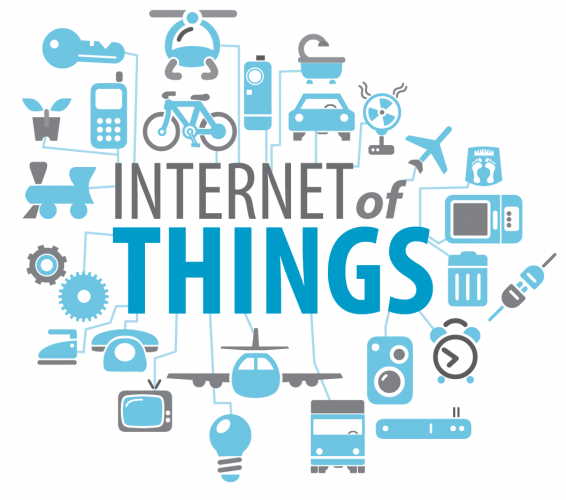
\includegraphics[scale=0.5]{98_Bilder/02_Grundlagen/iot}
  \caption[Symbolbild Internet of Things]{Internet of Things: Vernetzte Geräte bilden ein Internet der Dinge}
  \footnotesize \url{http://kpcbweb2.s3.amazonaws.com/content/710/original_aefd15169aaebd3f037b5ed672db6de1.png}, 20.11.2015
\end{figure}

\section{Smartwatches}
Smartwatches sind kompakte Computersysteme, welche vom Benutzers am Handgelenk getragen werden kann. Diese sind meist mit einer oder mehreren drahtlos Technologie und verschiedenen Sensoren (Bewegungssensor, Lichtsensor, Herzfrequenzmesser) Aktoren (Bildschrim, Vibrationsmotor) ausgerüstet.
Diese Uhren unterstützen den Träger beim alltäglichen Leben. Gehören zur Gruppe der Wearables und damit zu einem essentiellen Bereich des IoT. \\\\
\begin{figure}[h]
  \centering
  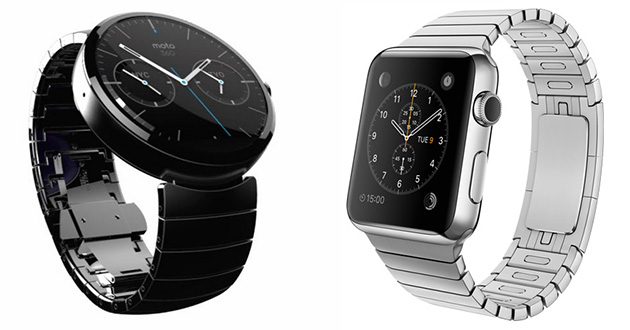
\includegraphics[scale=0.6]{98_Bilder/02_Grundlagen/androidwearapplewatch}
  \caption[Google's Android Wear und Apple Watch]{Motorola Moto360 mit Google's Android und Apple Watch mit iOS}
  \footnotesize \url{http://v-i-t-t-i.de/blog/wp-content/uploads/2014/09/android-wear-apple-watch.jpg}, 20.11.2015
\end{figure}


Mit einer Smartwatch können viele verschiedene Funktionalitäten mit einem Gerät abgedeckt werden.
\subsection{Beispiele}
\begin{tabular}{ll}
Pulsmessung: &	Überwachung des persönlichen Pulses \\
Bewegungen:	& Mögliche Bewegungen welche über das Handgelenk ermittelt werden können analysieren \\
Fitness: & Genaue Bewegungen können registriert und in kombination von Weg und ausgewertet werden \\
Informationen: & Der Träger kann Informationen empfangen welche auf seinem Smartphone ersichtlich sind
\end{tabular}

\subsection{Fachbereich Informatik}
Smartwatches gehören in den Bereich der Wearables. Dies ist ein fachübergreifendes Gebiet der Informatik, einige Fachgebiete:\\
- Ubiquitous Computing, die Rechnerallgegenwärtig \\
- Pervasive Computing, die Vernetzung von Alltagsgegenständen \\
- Mobile Computing, mobile Mensch zu Maschinen Kommunikation \\
- M2M, Machine-to-Machine, Informationsaustausch zwischen Zielgeräten \\
- IoT, Internet of Things, dass auf den vorhergehenden Fachbereichen basiert

\section{MQTT}

\section{siot.net}

Die Fachgruppe SIOT des Instituts RISIS der BFH konzipiert und entwickelt zusammen mit Industriepartner (AppModule AG) die Plattform siot.net, welche Sensoren und Aktoren weltweit mit IoT-Anwendungen verbindet.
Das Ziel dieser Plattform ist es sie zu industrialisieren um Klein und Mittlere Unternehmen (KMU) eine Möglichkeit zu geben ihre Sensoren und Geräte zu vernetzen. Dies soll vorteilhafterweise zu einem günstigen Preis möglich sein.
siot.net bietet für eine kleine Gebühr ein IoT-Center und die IoT Infrastruktur.
Konfiguration, Analyse, Verwaltung und Zuweisungen werlden alle im IoT-Center durchgeführt. Über das IoT-Center können alle Sensoren und Aktoren verknüpft und konfiguriert werden. Um die Daten auszuwerten und darzustellen wird ein Dashboard zur Verfügung gestellt. Die IoT-Infrastruktur beinhaltet einen MQTT Broker und die Definition, wie Meldungen auf den siot.net Broker angeliefert werden sollen.\\\\
\begin{figure}[h]
  \centering
  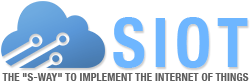
\includegraphics[scale=1.0]{98_Bilder/02_Grundlagen/siotnetLogo}
  \caption[siot.net Logo]{siot.net Plattform Logo}
  \footnotesize \url{http://siot.appmodule.rs:8000/images/logo.png}, 20.11.2015
\end{figure}
\subsection{IoT-Center}
